\chapter{Domain Driven Design} \label{sec:ddd}

\section{Ubiquitous Language (UL)}

\subsubsection{Card}

\textbf{Bedeutung:} Ein Objekt, welches von einer zuvor zufällig zusammengestellten Menge an Karten (Kartenstapel = CardDeck) 
erhalten (gezogen = draw) werden kann und dann durch einen Effekt den Spielverlauf beeinflusst.

\textbf{Begründung:} Card gehört zur UL, da es wichtig ist, dass Domänenexperten (die Spiel-Designer) und die Softwareentwicklern 
über Kartentypen und deren Effekte sprechen können, wenn neue solcher Karten hinzugefügt werden sollen, oder bestehende verstanden 
werden sollen. 


\subsubsection{AnimalEncounter}

\textbf{Bedeutung:} Eine Spielphase (= GamePhase) die durch den Karteneffekt einer Karte des Typs Tier (= Animal) 
ausgelöst wird und erst verlassen werden kann, in dem der RollDx-Befehl erfolgreich ausgeführt wird (Kampf gegen das Tier).

\textbf{Begründung:} AnimalEncounter ist Teil des UL, da die Spielphasen (vgl. \autoref{fig:phases}) im Software-Modell direkt und unverändert 
übernommen werden, um keine Übesetzung im Spielverlauf zwischen Software- und Kartenspiel haben zu müssen, was die Kommunikation sehr 
erschweren würde und Missverständnisse provozieren könnte. 


\subsubsection{Axe}

\textbf{Bedeutung:} Ein Objekt, welches das Tool- und Buildable-Interface implementiert, um so unter bestimmten Voraussetzungen 
erzeugt (crafted = hergestellt) werden zu können und im Spiel bessere Chancen (bonus damage = 
zusätzlicher Schaden) in der Encounter-Spielphase zu ermöglichen.

\textbf{Begründung:} Axe ist (wie das andere Tool \textit{Club} auch) Teil der UL, um die Klasse in der gemeinsamen Kommunikation mit den 
Domain-Experten identifizieren zu können. Dieses Objekt benötigt in jedem Fall einen Namen und statt z.B. \textit{StrongProbabilityIncreaser}
ist Axe griffiger und leichter zu merken - auch für die Entwickler. 


\subsubsection{Roll}

\textbf{Bedeutung:} Ein Verbundsobjekt aus einer Zufallsvariable eines diskreten natürlichzahligen Intervalls 
(Würfel-Art = Roll.type) und einer assoziierten Realisierung dieser Zufallsvariable (Augenzahl = Roll.roll).

\textbf{Begründung:} Roll als Würfelwurf ist in der UL, da es einem Würfeltyp eine (Augen-)Zahl zuordnet, wodurch eine technischere Bezeichnung, 
wie \textit{BoundedRandomInteger} keine Assoziation zu den verschiedenen Würfeln (vier-, sechs- und achtseitig) zulässt, 
die aber in der weiteren Entwicklung und Kommunikation mit den Domänenexperten wichtig sind. Außerdem beschreibt der Name den Zweck und 
den Ursprung, anders als der generische BoundedRandomInteger, der für alles stehen könnte und womit die Domänenexperten (und auch Entwickler)
deutlich weniger sich vorstellen und anfangen könnten.  


\section{Entities} \label{sec:entities}

\autoref{fig:entity} zeigt die \textit{GameState}-Klasse. Sie beinhaltet den ganzen Zustand des Spiels und wird genutzt 
um das Spiel zu speichern (und dann wieder zu laden), da alle relevanten Objekte hier verwurzelt sind. Dabei manipuliert die Game-Klasse
den GameState und nicht die Klasse sich selbst. Somit ist kein kaum Verhalten in der Klasse realisiert, was ein Punkt einer Entity ist. 
Diese Klasse befindet sich zwar nicht in der Domain-Schicht, aber hat sonst alle Merkmale einer Entity und aus gutem Grund. 
Die Identität eines GameStates soll nur von einer ID (hier der Surrogatschlüssel \textit{uuid} vom Typ \textit{UUID}) abhängen, 
da der Hauptzweck der Klasse die einfache Speicherbarkeit des Spielzustandes ist und ein genau gleicher Spielzustand von den Attributen her 
nicht als identisch angesehen werden soll, wenn die ID nicht stimmt, um unterschiedliche Speicherungen (selbst bei zufällig identischen Attributen)
unterscheiden zu können. Folglich wurden in GameState \textit{hashCode} und \textit{equals} im Sinne der Identität einer Entität überschrieben, 
sodass diese nur vom Surrogatschlüssel \textit{uuid} abhängen. Außerdem hat der GameState einen Lebenzyklus der insbesondere über 
die GamePhase und den GameStatus, aber auch sonstige Attribute, ausgedrückt wird. \\ 
Dies ist der einzige wirklich sinnvolle Einsatz von Entitäten im Programm, auch wenn es sich in der Application-Schicht befindet. 
Die Klasse \textit{Camp} wurde ebenfalls als Entität implementiert, wobei der Schlüssel allerdings nicht annähernd so eine wichtige 
und sinnvolle Bedeutung hat wie beim GameState. Darüber hinaus sollte es pro GameState auch nur ein und nicht mehrere Camps geben, 
weswegen das zum GameState gehörige Camp die gleiche uuid erhält, wie der GameState. Da es aber faktisch keine anderen Camps in einer 
Instanz der Applikation gibt, werden diese auch nie verglichen, weswegen diese Entität bisher wenig sinnhaft ist. 

\begin{figure}[H]
	\centering
	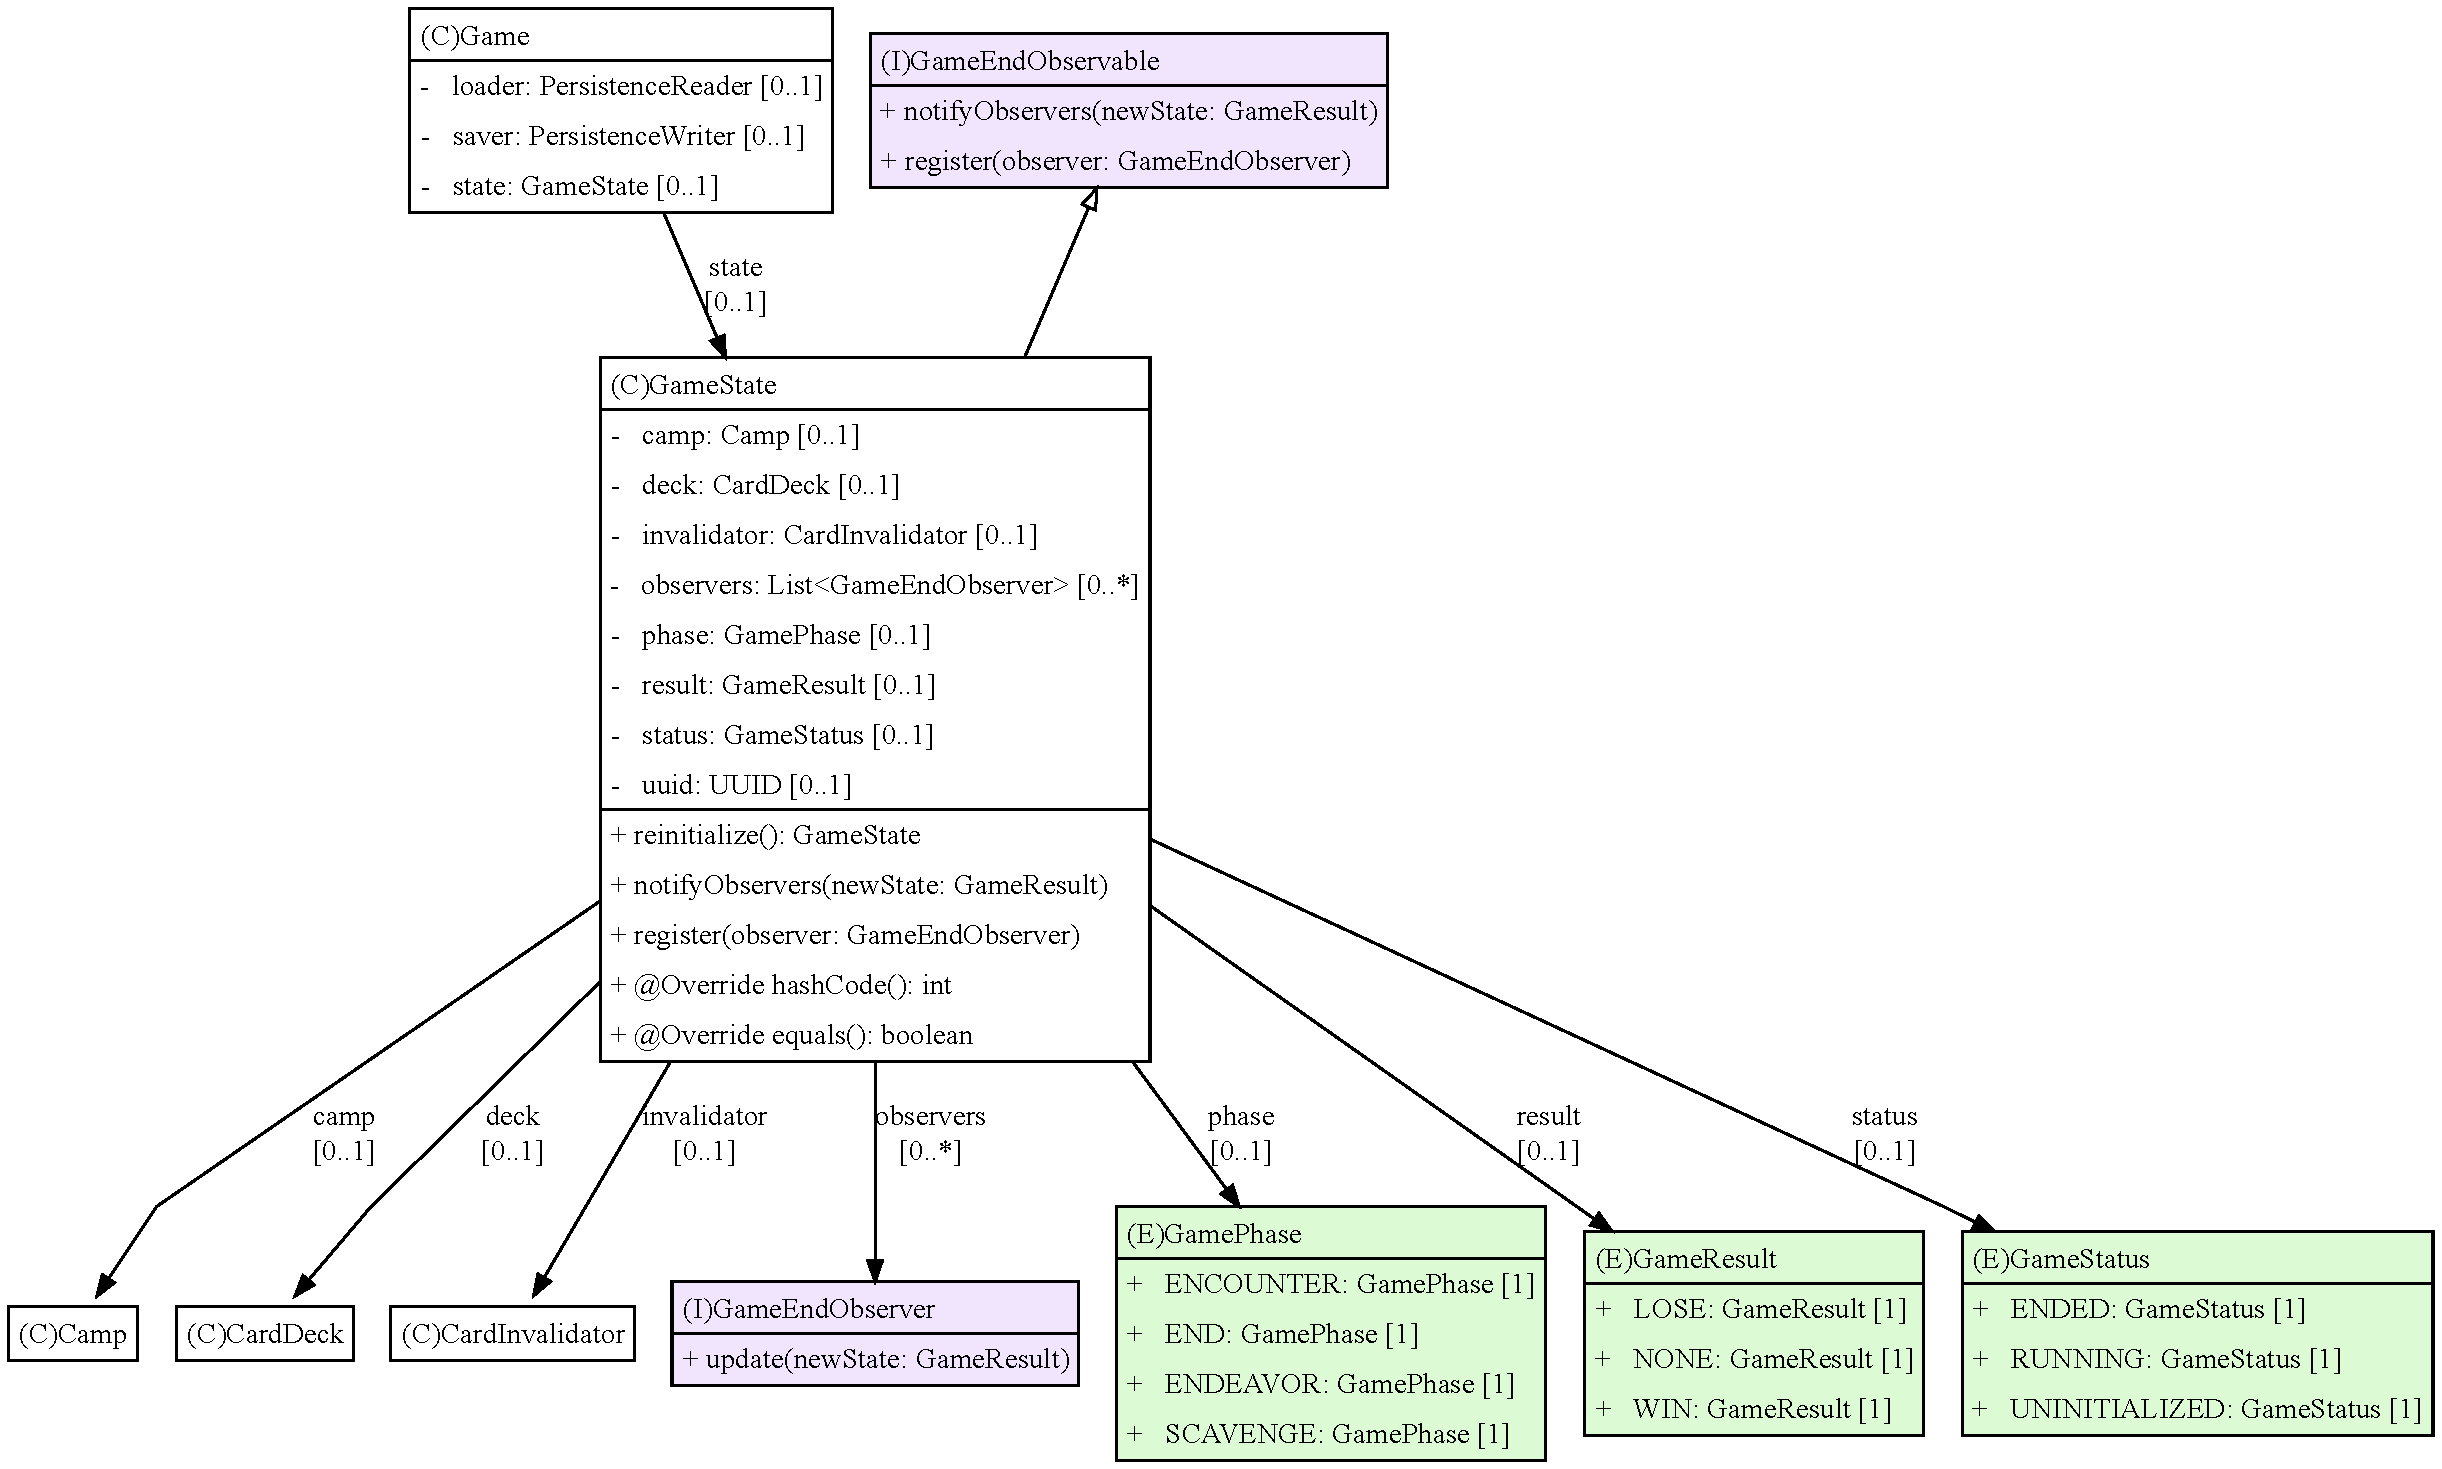
\includegraphics[width=1.05\textwidth]{Bilder/GameState_structure.pdf} 
	\caption{UML-Diagramm von \textit{GameState}.}
	\label{fig:entity}
\end{figure} 

\section{Value Objects (VO)}

\autoref{fig:vo} zeigt das VO \textit{Roll}, welches in Java als \textit{Record} implementiert ist. Demnach ist \textit{hashCode} und 
\textit{equals} bereits implizit entsprechend überschrieben, weswegen es nicht extra im Diagramm auftaucht. Das immutable VO 
Roll definiert eine Augenzahl (Roll.roll) für einen bestimmten Würfeltyp (Roll.type) und stellt die Domänen-Constraint sicher, 
dass Augenzahlen $a$ stets im Intervall von eins bis Seitenanzahl des Würfels $s$ liegen muss: $a \in [1, s];~ s \geq 1$. 
Dieser Constraint insbesondere wird dabei in das VO \textit{RollInteger} ausgelagert. Weiter bietet Roll verschiedene Methoden 
bereit um Verhalten bezüglich Rolls durchzusetzen. Beispielsweise kann die Augenzahl mit der Methode \textit{raisRollBy} 
erhöht werden, wobei ein neues Roll-Objekt mit der erhöhten Augenzahl aber maximal $Roll.roll = s$ zurückgegeben wird. \\
Roll wurde also als VO realisiert, da es so das Domänenkonzept kapselt und verdeutlicht, die Domänenregeln eingehalten werden, 
Domänenverhalten umgesetzt wird, keine Seiteneffekte auftreten und der Roll einfach mit anderen Rolls (z.B. dem benötigten Roll, 
um gegen ein bestimmtes Tier zu gewinnen (s. Klasse \textit{AnimalEncounter})) verglichen werden kann.

\begin{figure}[H]
	\centering
	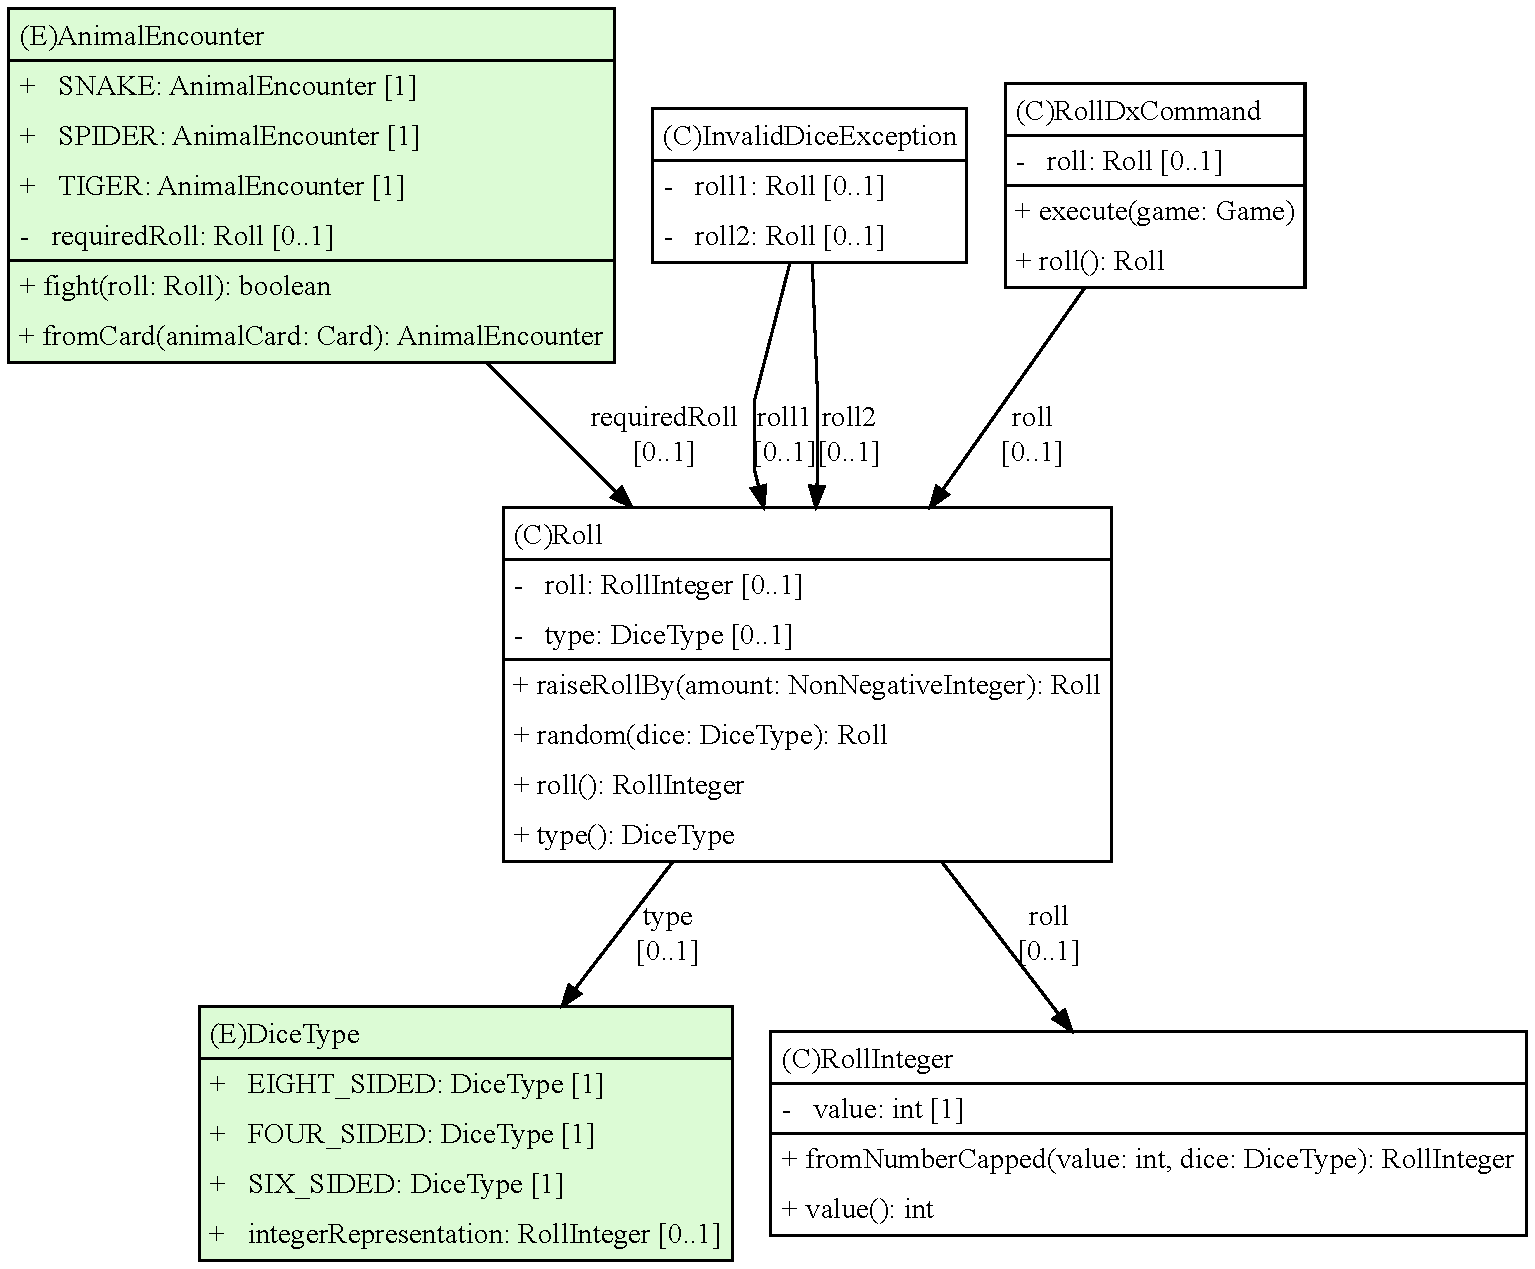
\includegraphics[width=0.8\textwidth]{Bilder/Roll_structure.pdf} 
	\caption{UML-Diagramm von dem Value Object \textit{Roll}.}
	\label{fig:vo}
\end{figure} 


\section{Repositories}

\autoref{fig:repository} zeigt das \textit{PersistenceReader}-Interface, was eine Art \enquote{Repository} auf Application-Layer-Ebene darstellt.
Wie schon in \autoref{sec:entities} angedeutet, spielt die Speicherung des GameStates die zentrale Rolle, um ein Spiel wiederherzustellen 
und später fortzusetzen. Es ergibt allerdings wenig Sinn, die einzelnen Aggregate der Domain-Schicht einzeln zu persistieren, den 
GameStatus, die GamePhase der Applikationschicht einzeln zu persistieren und dann später beim Laden zusammenzupflücken und 
einzeln wieder zusammenzubauen. Um das Spiel zu Speichern muss lediglich der GameState (der alle vorher genannten Objekte enthält) 
gespeichert werden. Dieser ist aber - und aus gutem Grund - Teil der Applikationsschicht, weswegen PersistenceReader per Definition
erst mal kein Repository sein kann (Repository-Interfaces müssen im Domain-Code definiert sein). Hier ist es aber sinnvoll nicht den 
puristischen Ansatz zu wählen, sondern die Konzepte etwas aufzuweichen, sodass PersistenceReader ein Repository darstellt, 
um den GameState zu lesen. \\
Das Repository ist nötig, um geringe Kopplung (vgl. \textit{Persistence\underline{Writer}} aus \autoref{sec:low-coupling}) zu gewährleisten, 
das OCP und die Dependency Rule einzuhalten. Somit kann die Implementation des PersistenceReader in der Plugin-Schicht beliebig getauscht werden,
ohne dass die höheren Schichten (Applikation und Domain) etwas davon wissen müssen oder gar von den Details abhängen müssen und 
stattdessen von der Abstraktion abhängen können. 

\begin{figure}[H]
	\centering
	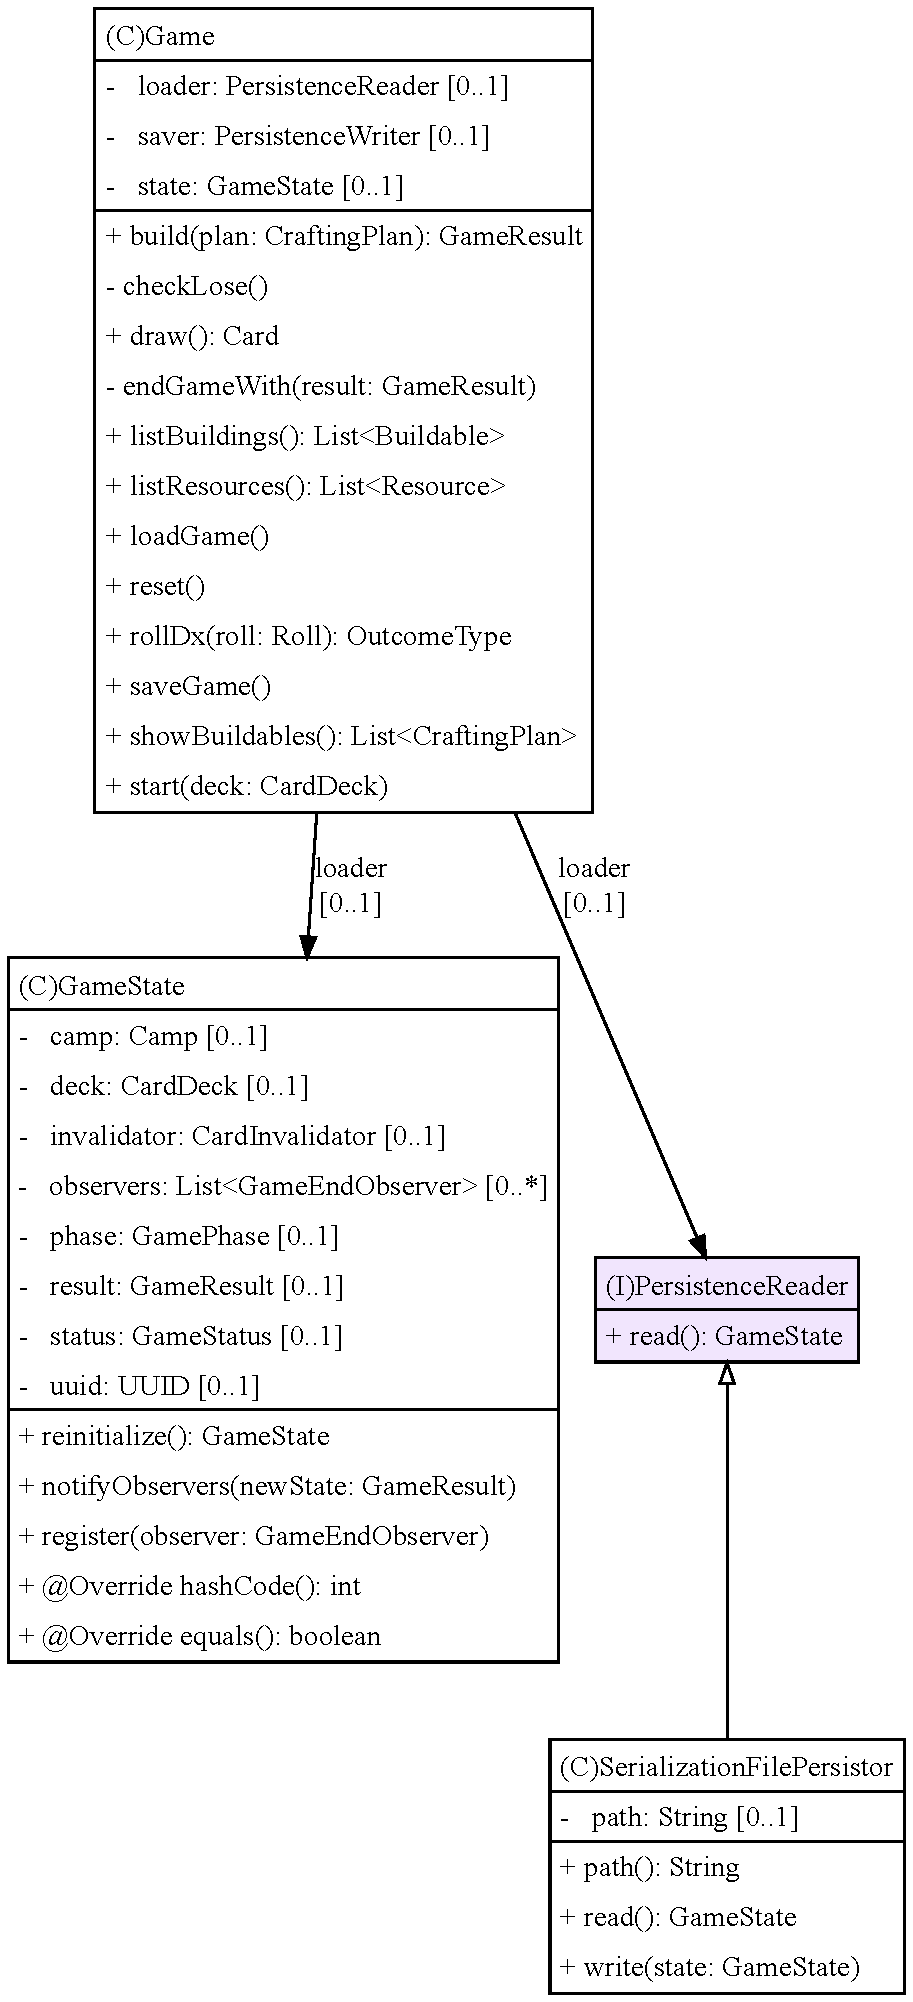
\includegraphics[width=0.5\textwidth]{Bilder/PersistenceReader_structure.pdf} 
	\caption{UML-Diagramm von dem Repository \textit{PersistenceReader}.}
	\label{fig:repository}
\end{figure} 

\section{Aggregates}

\autoref{fig:aggregate} zeigt das \textit{crafting}-Aggregat mit der Root-Entity \textit{Camp}. Es ist deutlich zu sehen,
dass Zugriff auf das Aggregat durch außenstehende Klassen \underline{nur} über die Root-Entity Camp möglich ist.
Hierfür bietet Camp öffentliche Methoden an, die lediglich an die anderen Klassen des Aggregats delegieren.
Dadurch können die Domain-Regeln, die sich auf das Aggregat beziehen zentral in den öffentlichen Methoden von Camp überprüft werden.
Außerdem werden die Zugriffe auf das Crafting-Aggregat und damit auch die Crafting-Funktionalität vereinfacht und die Objektbeziehungen 
werden entkoppelt, dadurch, dass für außenstehende Klassen nur das Camp existiert als Kopplungspartner und die Komplexität im 
Inneren des Aggregats versteckt wird. 

\begin{figure}[H]
	\centering
	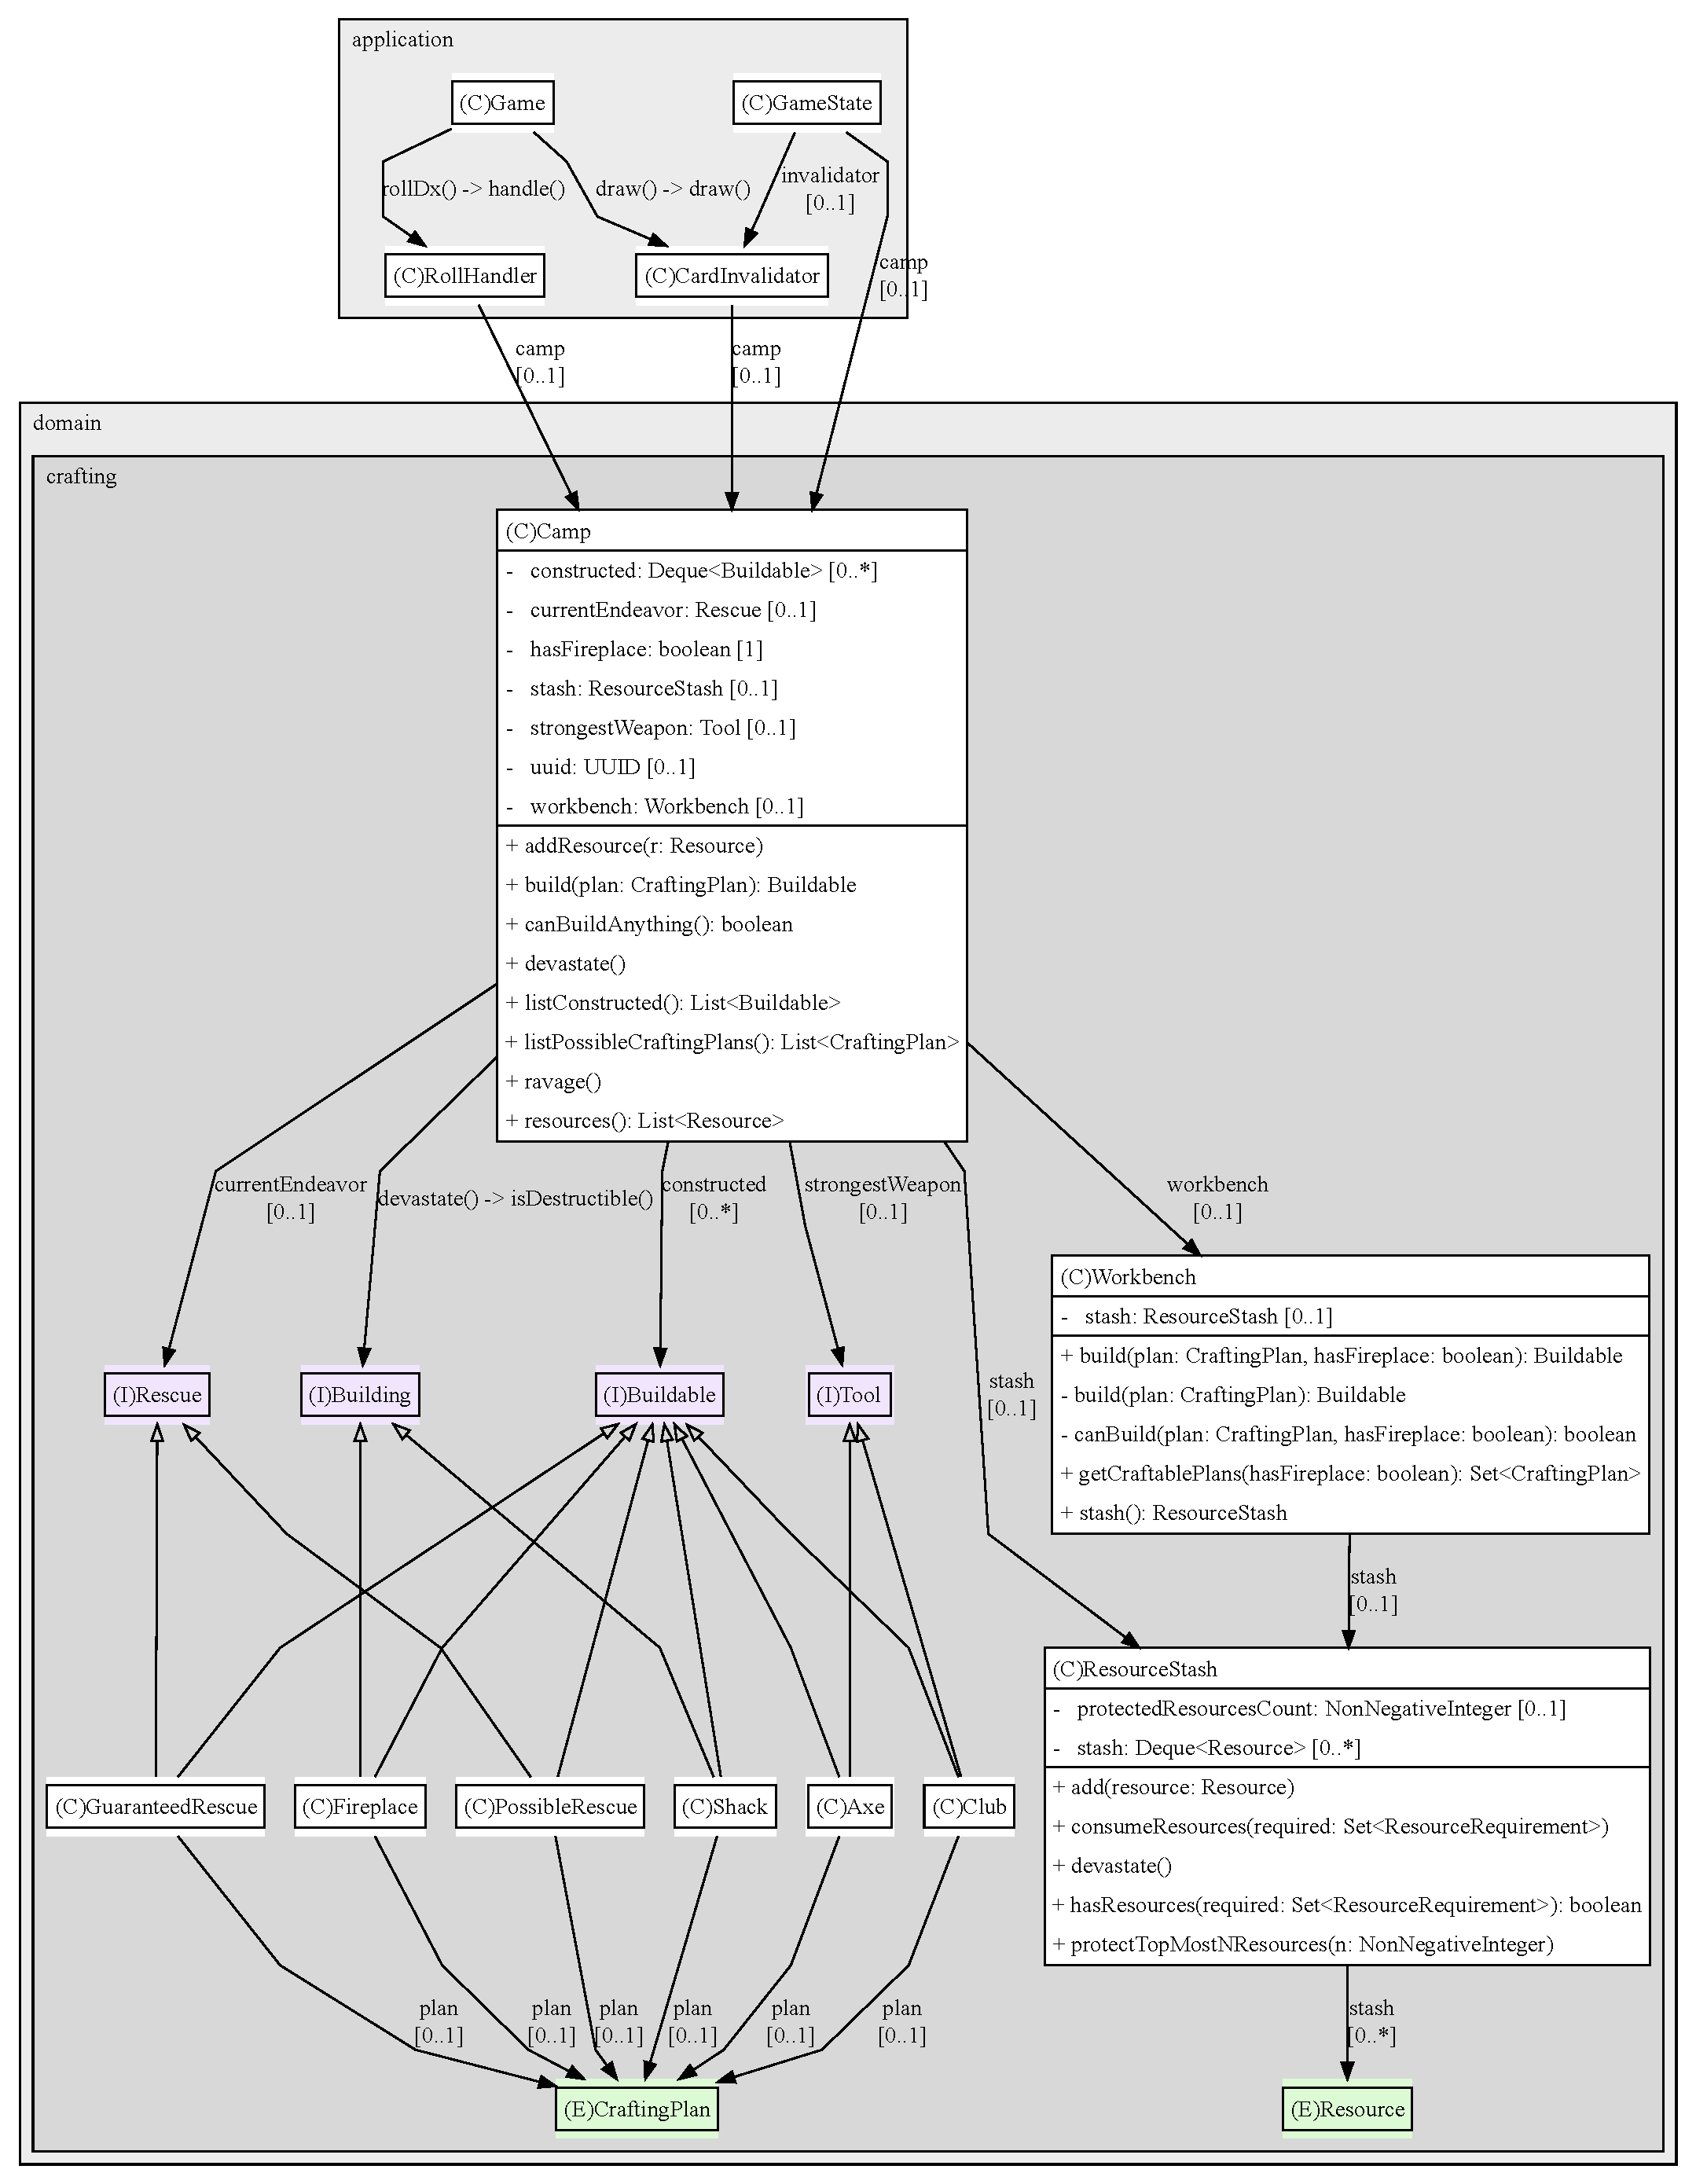
\includegraphics[width=1.05\textwidth]{Bilder/Camp_entity_structure.pdf} 
	\caption{UML-Diagramm vom \textit{crafting}-Aggregat mit \textit{Camp} als Root-Entity.}
	\label{fig:aggregate}
\end{figure} 

